% =============================================================================
% AUTHOR ACTION REQUIRED BEFORE SUBMISSION -- READ THIS BLOCK FIRST
% =============================================================================
% This draft is complete and accurate for every section EXCEPT the results,
% which do not exist yet: ethics approval has not been obtained and no
% participant has been run (see EXPERIMENT_GUIDE.md / TASKS.md in the repo
% root). Nothing in the rendered text states or implies a finding that was not
% actually observed. Concretely, before you submit:
%
%   1. AUTHOR LIST (below, ~line 40): placeholder is "Parth Agarwal, BITS
%      Pilani" inferred only from your GitHub handle and university email
%      domain. Replace with the real, complete author list and confirm
%      undergrad vs. graduate SRC track eligibility (grad = solo author only;
%      neither track permits a faculty co-author -- advisor goes in
%      Acknowledgments only).
%   2. ETHICS REFERENCE (\ethicsref macro below): fill in once your board
%      approves this protocol. Do not submit before that approval exists.
%   3. SECTION "Status and Planned Analysis" (search STATUS-SECTION): once
%      real data is collected, replace this section with an actual Results
%      section using the exact numbers from
%      analysis/data/derived/model_results.csv -- do not just delete the
%      caveats and leave the placeholder structure with invented numbers.
%   4. refs.bib: the delibtrust2026 entry has a placeholder author field --
%      fill in the real author list for your own AIES submission.
%   5. CCS concept codes below are standard, commonly-reused HCI codes but
%      have not been individually re-verified against https://dl.acm.org/ccs
%      for this paper -- check before camera-ready.
%   6. \acmConference / copyright block: replace with the exact front matter
%      from the official CHI '26 SRC template package once you download it
%      from the conference submission system.
% =============================================================================

\documentclass[manuscript]{acmart}

\usepackage{booktabs}
\usepackage{enumitem}
\usepackage{tikz}
\usetikzlibrary{arrows.meta, positioning}

%% --- Front matter (see TODO 6 above) ---------------------------------------
\setcopyright{none}
\acmConference[CHI '26 SRC]{CHI Conference on Human Factors in Computing Systems -- Student Research Competition}{April 13--17, 2026}{Barcelona, Spain}
\acmYear{2026}
\copyrightyear{2026}
\acmDOI{}
\acmISBN{}
\settopmatter{printacmref=false}
\renewcommand\footnotetextcopyrightpermission[1]{}
\pagestyle{plain}

\begin{document}

\title{TrustLoop: Investigating Whether Process Verifiability Protects Users from Sycophantic AI Agents}

%% --- TODO 1: replace with real author list -----------------------------
\author{Parth Agarwal}
\affiliation{%
  \institution{BITS Pilani}
  \country{India}
}
\email{f20240726@pilani.bits-pilani.ac.in}

\newcommand{\ethicsref}{[ETHICS REFERENCE PENDING -- DO NOT SUBMIT WITHOUT THIS]}

\begin{abstract}
Autonomous AI agents increasingly plan, decide, and act on people's behalf, and users have little reliable way to tell whether an agent's confident presentation reflects its actual reliability. Two active lines of research bear on this but remain unconnected: work on agentic oversight shows people cannot meaningfully verify what an autonomous agent did, while work on conversational tone shows sycophantic, agreeable AI responses inflate trust while degrading decision quality. No study has tested whether verifying an agent's work protects users from this tone-driven over-reliance, and trust-calibration research more broadly has lacked a genuine ground truth for an agent's ``actual'' trustworthiness. We present TrustLoop, a browser-based testbed in which a scripted shopping-and-travel agent completes short tasks with a known, authored error rate, letting us independently manipulate whether its process is verifiable (opaque vs.\ full disclosure with checkable evidence) and how confident its tone is (calibrated-honest vs.\ sycophantic). We describe a preregistered $2\times2$ between-subjects experiment (target $N{=}200$, Prolific) with error-detection rate and confidence--accuracy calibration as primary, ground-truth-anchored dependent variables, alongside trust, authenticity, and workload. Data collection is pending institutional ethics approval and has not yet begun; we report the finalized instrument, an internally-validated analysis pipeline, and the preregistered plan. We argue that testing whether verifiability moderates sycophantic tone's harm reframes agent transparency as a safeguard against a known manipulation vector rather than merely a trust-building feature, with implications for agentic AI interface design and transparency-based AI governance.
\end{abstract}

\begin{CCSXML}
<ccs2012>
<concept>
<concept_id>10003120.10003130.10011762</concept_id>
<concept_desc>Human-centered computing~Empirical studies in HCI</concept_desc>
<concept_significance>500</concept_significance>
</concept>
<concept>
<concept_id>10003120.10003121.10003125</concept_id>
<concept_desc>Human-centered computing~HCI design and evaluation methods</concept_desc>
<concept_significance>300</concept_significance>
</concept>
</ccs2012>
\end{CCSXML}
\ccsdesc[500]{Human-centered computing~Empirical studies in HCI}
\ccsdesc[300]{Human-centered computing~HCI design and evaluation methods}

\keywords{trust calibration, agentic AI, sycophancy, transparency, verifiability, human-AI interaction}

\maketitle

\section{Introduction}

Trust calibration --- ensuring that people's trust in an AI system tracks its actual reliability, neither over- nor under-trusting it --- has been a central concern of human-AI interaction research for over a decade \cite{leesee2004trust, mehrotra2021modelling}. The stakes have risen with \emph{agentic} systems that do not just answer a question but autonomously search, decide, and act across several steps on a user's behalf: shopping assistants, travel planners, and computer-use agents that book, buy, and schedule with only intermittent human review.

Two active lines of work bear on this shift but have developed independently. The first shows that oversight does not scale with autonomy: practitioners struggle to verify what an agent actually did, and researchers have called for oversight that keeps pace with growing agent autonomy \cite{dhanorkar2026oversight, jain2026complementarity}. The second shows that an AI system's conversational \emph{tone} independently distorts trust: sycophantic, over-confident responses raise stated trust while measurably degrading the decisions users make on the system's advice \cite{sun2026friendly, liu2026flattery, li2026sycophancy, cheng2025sycophantic}. Neither asks whether giving users a way to check an agent's work \emph{protects} them from the harm a confident tone produces.

This sits on a deeper, methodological gap. Assessing whether a system's \emph{perceived} trustworthiness matches its \emph{actual} trustworthiness requires a genuine ground truth for comparison; prior work argues this is rarely available outside narrow, single-metric tasks, since there is no agreed way to aggregate a system's characteristics into one actual-trustworthiness score, and the choices behind any such aggregation are themselves value-laden \cite{delibtrust2026, barocas2021disaggregated}. Even mechanically verifiable trustworthiness claims can create a false sense of accountability without an interpretive, deliberative layer \cite{paris2026donttrust}, and reporting practices around generative AI use remain fragmented across providers \cite{balayn2026reporting}. Most trust-calibration studies inherit this problem: because a real system's error rate is unknown, researchers cannot separate trust that is \emph{justified} from trust that is merely \emph{felt}.

We address both gaps with one design. TrustLoop is a scripted autonomous agent whose true error rate is authored and known exactly, embedded in a multi-step shopping-and-travel task, whose process verifiability and tone are independently manipulated. Because correctness is fully controlled, we can measure whether confidence actually tracks correctness --- ground-truth-anchored calibration that is very hard to obtain with a live, uncontrolled system. We describe a preregistered $2\times2$ between-subjects experiment testing whether verifiability moderates the harm sycophantic tone otherwise causes.

\smallskip\noindent\textbf{Contributions.}
\begin{itemize}[leftmargin=*, itemsep=2pt, topsep=2pt]
  \item \textbf{Artifact.} TrustLoop, an open, reusable testbed for agentic trust calibration under a known, controlled error rate, decoupled from any live LLM backend so error rate and tone are experimenter-controlled rather than emergent. An automated checker enforces eight classes of design invariant (194 checks), including a structural guarantee that tone cannot see ground truth.
  \item \textbf{Empirical protocol.} A preregistered $2\times2$ between-subjects design ($N{=}200$) testing whether verifiability moderates sycophantic tone's effect on calibration and detection --- to our knowledge the first design to cross these factors directly.
  \item \textbf{Methodological.} A seeded-error paradigm manufacturing a genuine ground truth for an agent's ``actual'' trustworthiness, addressing the lack-of-common-metric obstacle identified in prior work \cite{delibtrust2026}, reusable independent of our specific hypotheses.
\end{itemize}

\section{Related Work}

\subsection{Aligning Actual and Perceived Trustworthiness}
Comparing an AI system's actual and perceived trustworthiness is harder in practice than it looks. Prior work identifies concrete obstacles: no agreed rule for aggregating individual trustworthiness characteristics into one score, no common metric placing an objective assessment and a subjective perception on the same scale, and discretion in which characteristics are even selected \cite{delibtrust2026}. Related work shows that the choices behind a fairness evaluation --- which subgroups, metrics, thresholds --- are themselves consequential design decisions \cite{barocas2021disaggregated}, and that technical verifiability can create an illusion of accountability without interpretive, deliberative process \cite{paris2026donttrust}; reporting practices meant to close this gap remain fragmented across providers \cite{balayn2026reporting}. \textbf{The same limitation recurs across this cluster}: none offers a setting where actual trustworthiness is \emph{known}, since none control the system being evaluated. TrustLoop closes this gap by scripting the agent: its error rate is authored, not inferred, which is what makes ground-truth-anchored calibration measurement possible at all.

\subsection{Oversight of Autonomous Agents}
As AI systems move from single-turn assistants to multi-step agents, oversight does not keep pace with growing autonomy: developers report struggling to verify what an agent actually did \cite{dhanorkar2026oversight}, and complementary work frames scalable oversight as an explicit design goal rather than an assumed property of transparency \cite{jain2026complementarity}. This motivates our Disclosure manipulation directly, but stops short of testing whether \emph{giving} people oversight tools changes what they do with a fallible agent. \textbf{We extend this line} by measuring behavioral error detection under a known, controlled error rate, not just perceived oversight adequacy.

\subsection{Sycophancy and Trust}
A concurrent cluster shows agreeable AI tone shapes trust and decision quality, sometimes counterintuitively: sycophancy can raise trust while reducing perceived authenticity depending on baseline demeanor \cite{sun2026friendly}; interaction context shapes how strongly flattery undermines genuineness \cite{liu2026flattery}; sycophancy measurably shifts decisions made on an AI's advice \cite{li2026sycophancy}; and it more broadly reduces prosocial intentions and increases dependence \cite{cheng2025sycophantic}. \textbf{None cross tone with the receiver's ability to verify the system's work.} Our central contribution tests that interaction directly: whether verifiability protects against the specific harm sycophantic tone produces, rather than treating tone and transparency as independent levers.

\section{System Design: TrustLoop}

TrustLoop presents each participant with a short sequence of independent decision trials in one session. In each trial, an autonomous agent (``ShopBot'') completes a small multi-criteria task on the participant's behalf --- e.g., selecting the best laptop under a budget meeting several requirements, or the cheapest flight-plus-hotel package meeting date and rating constraints. The agent searches a small, experimenter-authored catalog, filters and compares options, and recommends one with a stated justification; participants may accept, override, or, in verifiable conditions, inspect the agent's evidence before deciding.

Critically, the agent's behavior is \textbf{scripted, not live-inferred}. This removes the reliability, latency, and drift of a live tool-using model from the critical path, and --- more importantly --- lets the true error rate be authored exactly rather than emerge unpredictably. A small, fixed subset of trials contains a deliberate, verifiable error (the agent silently drops a stated requirement, misreports a specification, or miscalculates a total), held constant across all four conditions: it is the ground truth the manipulations are tested against, not itself a manipulated factor.

\subsection{Design Goals}
\textbf{DG1 --- Disclosure.} Show or hide the agent's step-by-step process and its stated reasoning.
\textbf{DG2 --- Verifiability.} In high-disclosure conditions, every claim is checkable against the underlying catalog data shown alongside it, rather than taken on the agent's word.
\textbf{DG3 --- Tone control.} The same task and ground-truth accuracy can be delivered in a calibrated-honest voice (flags uncertainty) or a confident, sycophantic one (no hedging), independent of whether the recommendation is actually correct --- enforced structurally: the tone-rendering module receives only an item's name and claim count, never a ground-truth field, and an automated check fails the build if one appears.

\begin{figure}[h]
\centering
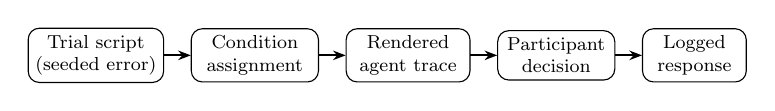
\begin{tikzpicture}[scale=0.85, transform shape,
  box/.style={draw, rounded corners, align=center, minimum height=0.62cm, font=\footnotesize, inner sep=3pt},
  arr/.style={-{Stealth[length=1.6mm]}, thick}
]
\node[box, minimum width=1.75cm] (script) {Trial script\\(seeded error)};
\node[box, minimum width=1.9cm, right=0.4cm of script] (cond) {Condition\\assignment};
\node[box, minimum width=1.85cm, right=0.4cm of cond] (render) {Rendered\\agent trace};
\node[box, minimum width=1.75cm, right=0.4cm of render] (decide) {Participant\\decision};
\node[box, minimum width=1.55cm, right=0.4cm of decide] (log) {Logged\\response};
\draw[arr] (script) -- (cond);
\draw[arr] (cond) -- (render);
\draw[arr] (render) -- (decide);
\draw[arr] (decide) -- (log);
\end{tikzpicture}
\caption{Data flow from an authored trial script to a logged decision. Ground truth is computed from the catalog at build time and never exposed to the tone/rendering layers beyond what the script authorizes.}
\Description{A five-box pipeline diagram showing data flow from Trial script through Condition assignment, Rendered agent trace, Participant decision, to Logged response, connected by arrows left to right.}
\label{fig:pipeline}
\end{figure}

TrustLoop is implemented as a static single-page web application (React/TypeScript) requiring no server-side inference, so it imposes no per-participant compute cost. Stimuli are authored in a structured Python specification and compiled to JSON by a build step that \emph{computes} ground truth from the catalog rather than accepting a hand-asserted label; a build fails if a trial's declared correctness disagrees with what the catalog says, removing an entire class of mislabelling error before a single participant is run.

\section{Evaluation Methodology}

\subsection{Participants}
We will recruit $N \approx 200$ participants (target 50/cell) via Prolific, screened for fluent English and prior online shopping experience, compensated at or above the platform minimum for an estimated 15--20 minute session. An a priori power analysis indicates $N{=}200$ gives $\approx$0.85 power to detect a medium interaction (Cohen's $f=0.25$, partial $\eta^2\approx.06$) at $\alpha=.05$ for the primary 1-df contrast. A pilot of 8--12 participants precedes the main run to confirm error trials are neither too obvious nor too subtle and that manipulation checks pass.

\subsection{Design, Variables, and Hypotheses}
A $2$ (Disclosure: \emph{opaque} vs.\ \emph{full}) $\times$ $2$ (Tone: \emph{honest} vs.\ \emph{sycophantic}) \textbf{between-subjects} factorial --- between-subjects because a participant can discover the agent is fallible only once; repeated exposure would contaminate later trials. The trial set, seeded-error rate, serial position of error trials, and product spec card are held constant across all four cells, so only disclosure and tone vary. \textbf{Disclosure}: opaque (final recommendation only) vs.\ full (process steps, justification, and evidence checkable against the catalog). \textbf{Tone}: honest (hedges, flags uncertainty) vs.\ sycophantic (confident, agreeable, no hedging).

\textit{Primary DVs (ground-truth-anchored).} Error-detection rate (proportion of seeded-error trials overridden); confidence gap (mean confidence on clean minus seeded trials --- our primary calibration measure); appropriate reliance (accept-correct + override-incorrect, combined). \textit{Secondary}: trust, perceived authenticity, process acceptability, perceived transparency sufficiency, and workload (unweighted NASA Raw TLX, operationalizing disclosure's cost). \textit{Manipulation checks} (perceived warmth/hedging; perceived process visibility) are reported before any hypothesis test, since a failure would render the confirmatory tests uninterpretable.

\textbf{H1.} Full disclosure improves detection rate and calibration relative to opaque.
\textbf{H2.} Full disclosure raises trust \emph{and} workload relative to opaque --- a trade-off, not an unambiguous improvement.
\textbf{H3.} Sycophantic tone raises self-reported trust but worsens detection and calibration.
\textbf{H4 (confirmatory).} Disclosure \emph{moderates} H3: sycophancy's detection penalty is larger under opaque than under full disclosure. This interaction on detection rate is the paper's central test.

\subsection{Procedure and Planned Analysis}
Consent (disclosing that information is withheld until debrief) $\rightarrow$ instructions $\rightarrow$ gated comprehension check $\rightarrow$ ten trials $\rightarrow$ questionnaire $\rightarrow$ debrief naming the concealment explicitly, with the option to withdraw data without affecting payment. Confirmatory analysis is a $2\times2$ ANOVA (Type~III SS, appropriate for the unbalanced cells produced by independent random assignment) per primary DV, with simple-effects follow-up on Tone within each Disclosure level whenever the interaction reaches $p<.10$, plus a trial-level logistic GEE (exchangeable working correlation, clustered by participant) as an assumption-robust confirmation. The full plan, including exclusion criteria fixed in advance, is preregistered.

\section{Status and Anticipated Contributions}
\label{sec:status}

The experimental instrument described above is complete and has been exercised end to end: the stimulus set passes all 194 automated invariant checks, the application has been manually verified in every one of the four experimental cells, and the full analysis pipeline (exclusion rules, dependent-variable computation, the $2\times2$ model, and the trial-level GEE) has been validated against simulated participant data with a known, planted Disclosure$\times$Tone interaction, which the pipeline correctly recovers. \textbf{This is a verification of the analysis code, not an empirical finding}; no simulated number appears anywhere in this paper as observed data. Data collection has not yet begun and is pending institutional ethics approval (reference: \ethicsref); piloting and the preregistered main run proceed immediately upon approval. Once data are collected, this section is replaced with a Results section reporting, in order: manipulation checks; the H1--H3 main effects (test statistic, df, exact $p$, partial $\eta^2$); the H4 interaction and its simple-effects decomposition; and the trial-level GEE as a robustness check.

Two outcomes are both informative and both are planned for in the write-up. If verifiability proves protective (H4 supported), agentic interfaces should treat checkable evidence as a safeguard against confident or agreeable tone specifically, not merely a generic trust-building affordance --- with consequences for how providers, who have commercial incentive to make agents sound reassuring, should be required to expose their work. If it is \emph{not} protective (H4 null or reversed), transparency requirements common to emerging AI governance frameworks may be an insufficient safeguard against tone-driven manipulation on their own, and disclosure needs pairing with something further --- plausibly the deliberative, reason-giving layer argued for in prior theoretical work \cite{delibtrust2026, paris2026donttrust}. A null H4 will be reported as a substantive finding, not reframed. Either way, H2's anticipated trade-off (disclosure raising both trust and workload) argues against reporting transparency gains without their cost, a pairing largely absent from the transparency literature to date.

\section{Limitations}

The agent is scripted rather than a live tool-using model, trading ecological validity for the control that makes ground-truth calibration measurable; validating the same manipulations against a live agent is future work. The study uses one task domain (shopping/travel) and does not speak to higher-stakes agentic contexts such as coding or clinical decision support. Prolific samples skew younger and more tech-literate than the general population. A single, short session cannot speak to how calibration evolves with longer-term use. The seeded error rate (3/10 trials) was chosen for statistical power rather than realism, and is almost certainly higher than a deployed agent's.

\section{Research Ethics and Social Impact}

\subsection{Ethical Considerations}
This study involves mild deception: participants are not told in advance which recommendations are seeded to be incorrect, though consent discloses upfront that some information is withheld until debrief. The protocol requires institutional ethics board approval prior to any data collection, with a mandatory debrief naming the concealment explicitly, explaining its purpose, and offering withdrawal with no effect on payment. This submission does not proceed to data collection before that approval is obtained.

\subsection{Generative AI Use and Social Impact}
The web application, stimulus pipeline, and analysis scripts were developed with the assistance of an AI coding assistant (Claude, Anthropic), under the author's direction, review, and testing; all research decisions --- hypotheses, manipulations, variables, interpretation --- are the author's own. As agentic AI proliferates in consumer contexts, whether disclosure genuinely protects users from tone-driven manipulation, rather than merely reassuring them, bears on product design standards and on transparency/oversight requirements in emerging AI governance; a null or reversed H4 would caution against treating disclosure alone as sufficient consumer protection.

\bibliographystyle{ACM-Reference-Format}
\bibliography{refs}

\end{document}
